\subsection{Pulse Width Modulation} \label{ssec:pwm}
	
	Pulse Width Modulation (PWM), is a way of modulation for encoding information on a pulse train signal. There are many ways of encoding and extracting this message out of the PWM signal and this type of modulation can be used for a wide varriety of applications such as controlling the charge delivered to a load and transmitting information \cite{standard19961037c}. PWM signals have a fixed high and a fixed low voltage level, there are two parameters that can be varried on a PWM signal: oscilation frequency and duty cycle. Figure \ref{fig:dutyCycle} shows how a the duty cycle affects a PWM signal. 

	\begin{figure}[htbp]
		\centering
			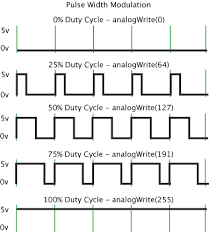
\includegraphics[scale=0.4]{figuras/fig-dutyCycle}
		\caption{Duty Cycle Examples \cite{fig-dutyCycle}}
		\label{fig:dutyCycle}
	\end{figure}

	Duty cycle can be defined mathematically by the Equation \ref{eqn:dutyCycle} \cite{james2001fundamentals}, where \textit{$D_{\%}$} is the duty cycle in percentage, \textit{PW} is the pulse width (pulse active time) and \textit{T} is the wave period. 

	\begin{equation}\label{eqn:dutyCycle}
		D_{ \left( \% \right) } =\frac{PW}{T}
	\end{equation}

	One useful way of using a PWM duty cycle variation is by enconding a analog voltage level proportional into it's percentage \cite{holmes2003pulse}, meaning that 100$\%$ duty cycle would represent maximum voltage amplitude and 0$\%$ the minimum voltage. This means it is possible to extract a analog voltage level by taking a PWM average level using a LPF \cite{alter2008pwm}, this is a practical way for designing digital to analog converters.
		
